%% comparative_genomics_intro.tex
%% Author: Leighton Pritchard
%% Copyright: James Hutton Institute
%% A brief description of the power of comparative genomics

% SUBSECTION: What you get back
% What you get back from assembly
\subsection{Computational Comparative Genomics}

% What computational comparative genomics gives you
\begin{frame}
  \frametitle{The Power of Comparative Genomics}
  Massively enabled by high-throughput sequencing, and the availability of thousands of sequenced isolates.\\[0.5cm]
  Computational comparisons more powerful and precise than experimental comparative genomics: \textbf{the ultimate microbial typing solution}\\[0.5cm]
  Three broad areas/scales:
  \begin{itemize}
    \item Comparison of bulk genome properties
    \item Whole genome sequence comparisons
    \item \textit{Comparison of features/functional components}
  \end{itemize}    
\end{frame}

% Bulk genome properties
\begin{frame}
  \frametitle{Bulk Genome Properties}
  Not taking sequence order/structure into account
  \begin{columns}[T]
    \begin{column}{5cm}
      \begin{itemize}
        \item Chromosome and plasmid counts
        \item Chromosome and plasmid sizes
        \item Nucleotide content
        \item $k$-mer content
      \end{itemize}    
      Classification/discrimination of sequences\\
    \end{column}
    \begin{column}{5cm}
      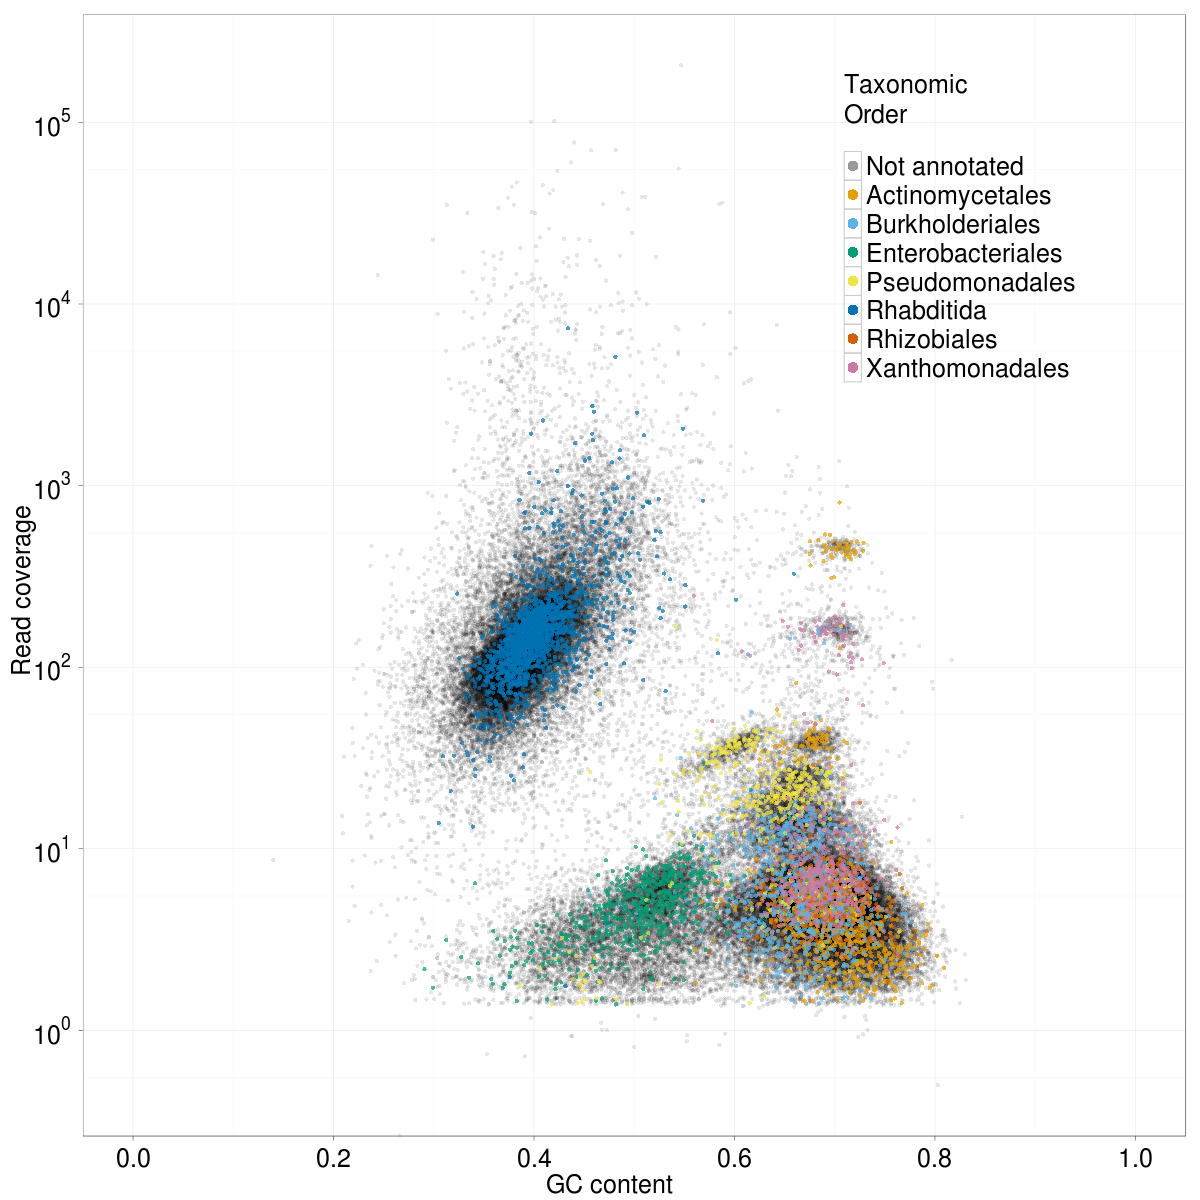
\includegraphics[width=1\textwidth]{images/blobology}
    \end{column}
  \end{columns}
\end{frame}

% Whole genome sequence comparisons
\begin{frame}
  \frametitle{Whole Genome Sequences}
  Introduces sequence order and structure
  \begin{itemize}
    \item Whole genome similarity
    \item Identification of sequence-similar regions
    \item Rearrangements
    \item Insertions/deletions
  \end{itemize}    
  Genome structure/evolution, and taxonomic classification.
  \begin{center}
    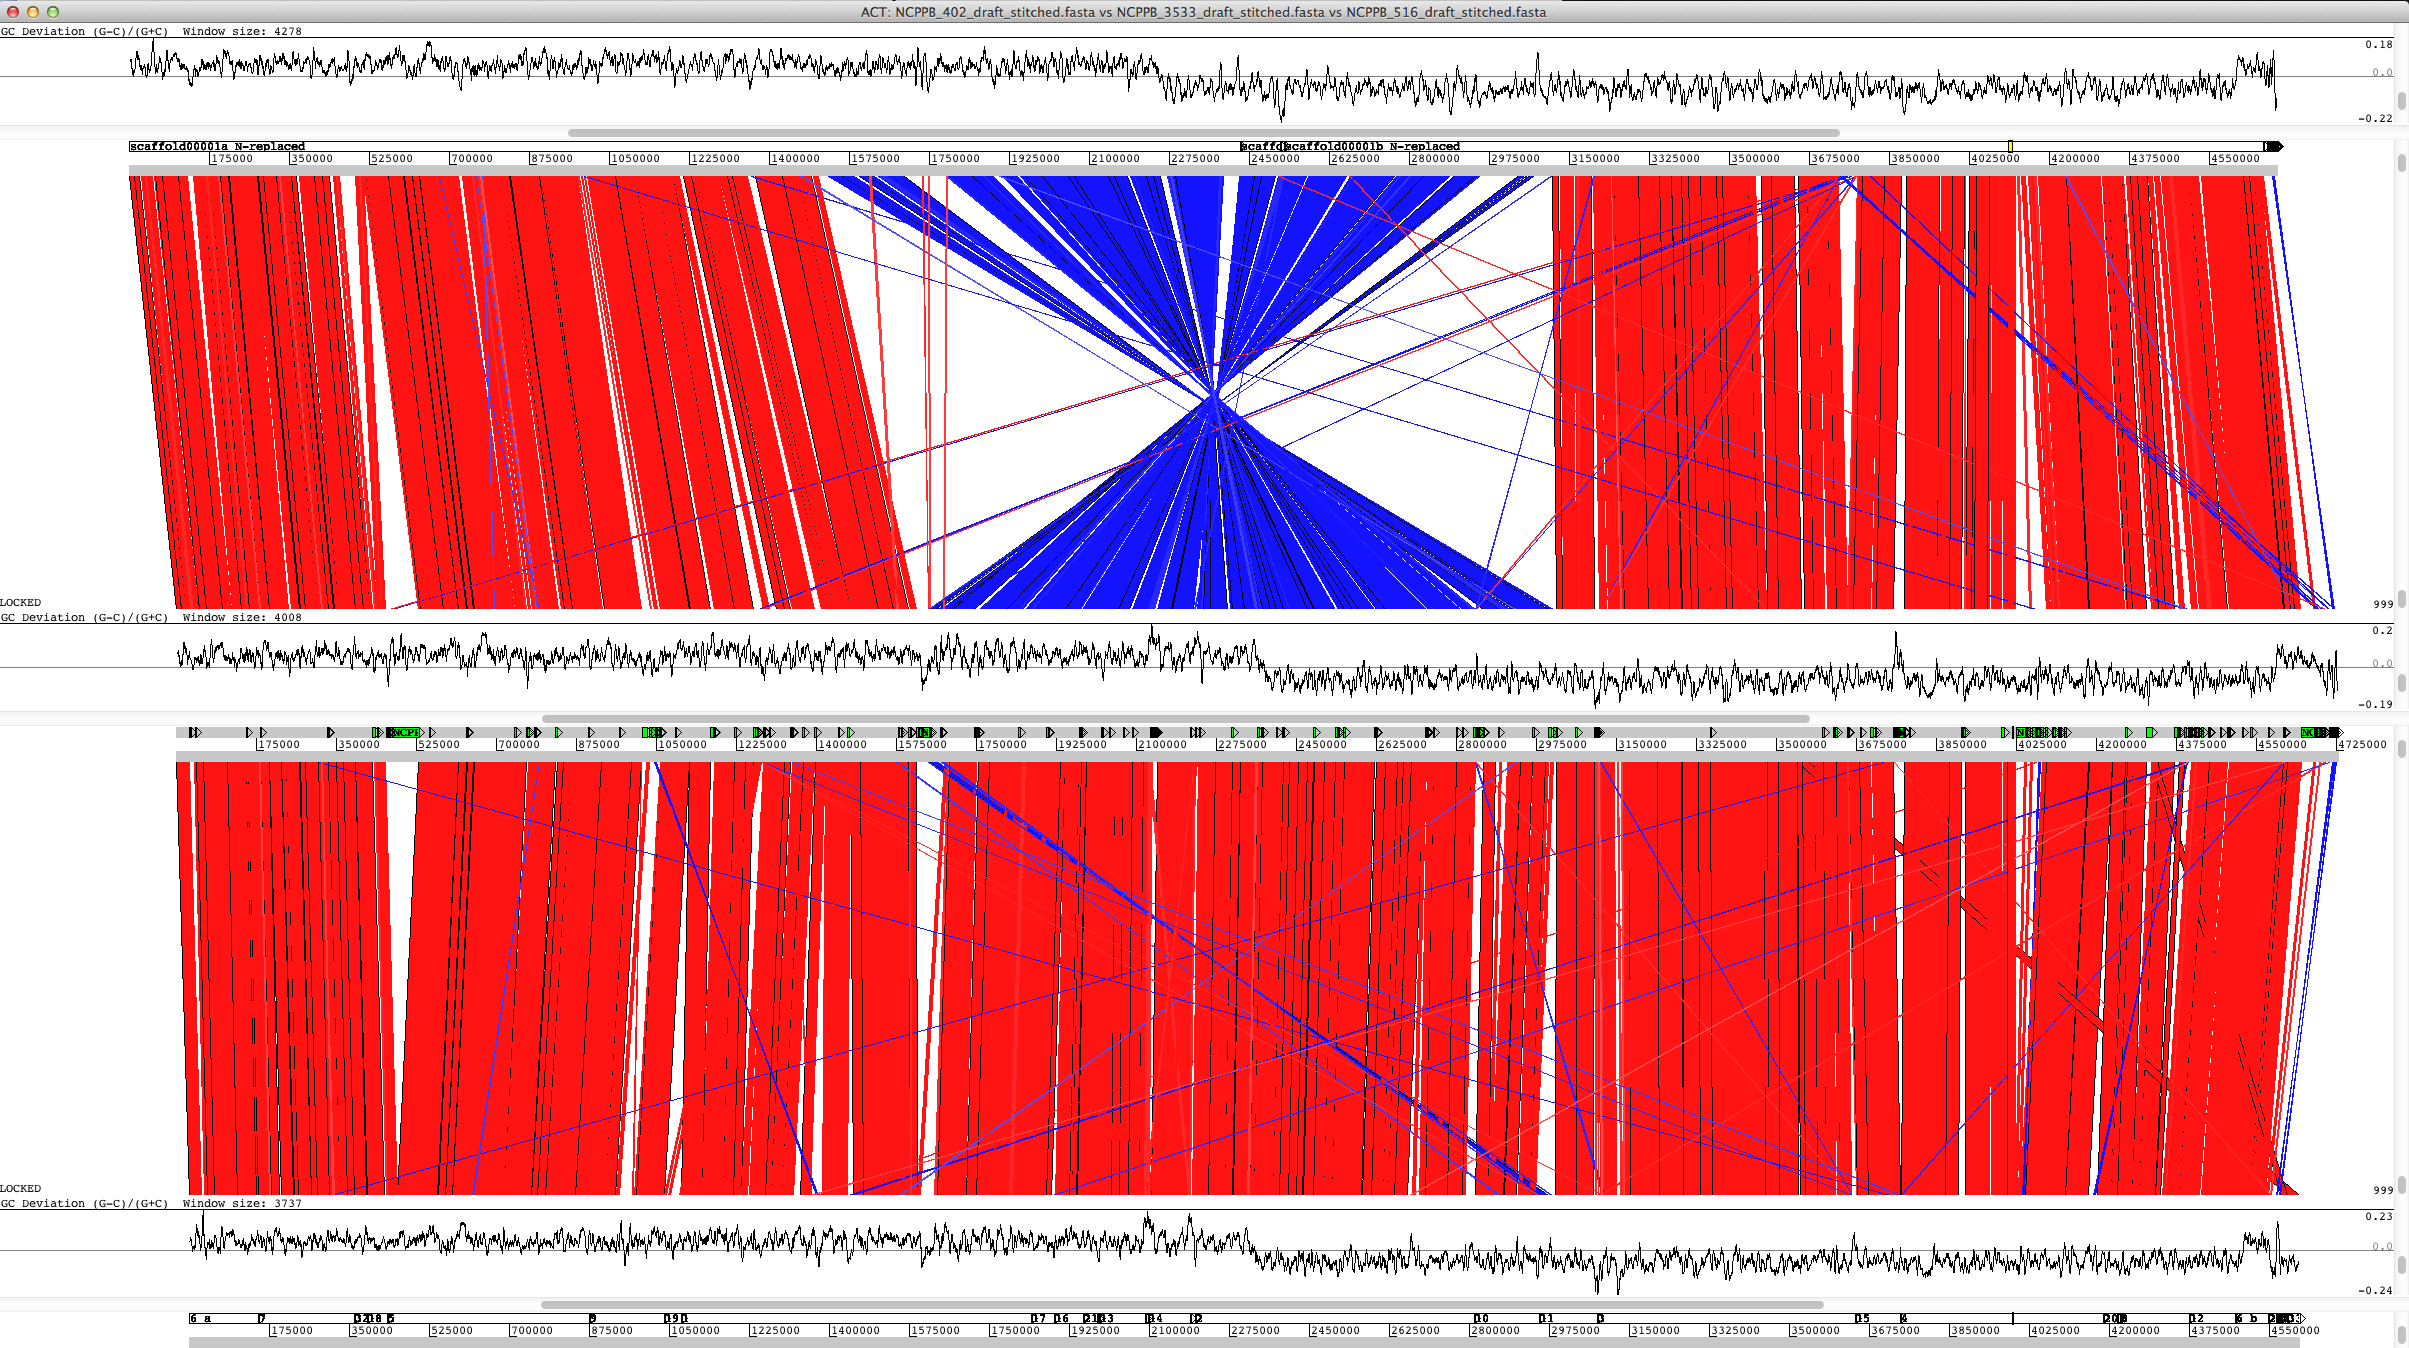
\includegraphics[height=0.4\textheight]{images/act_comparison}
  \end{center}  
\end{frame}

% Genome features and functional components
\begin{frame}
  \frametitle{Genome Feature Comparisons}
  Introduces functional elements, sequence subregions
  \begin{columns}
    \begin{column}{5.5cm}
      \begin{itemize}
        \item Numbers and types of features (genes, ncRNA, regulatory elements, etc.)
        \item Organisation of features (synteny, operons, etc.)
        \item Inference of functional/phenotypic differences
        \item Inference of selection pressure and adaptation
      \end{itemize}  
      Functional capacity, modifications/adaptations of biochemistry and phenotype  
    \end{column}
    \begin{column}{5cm}
      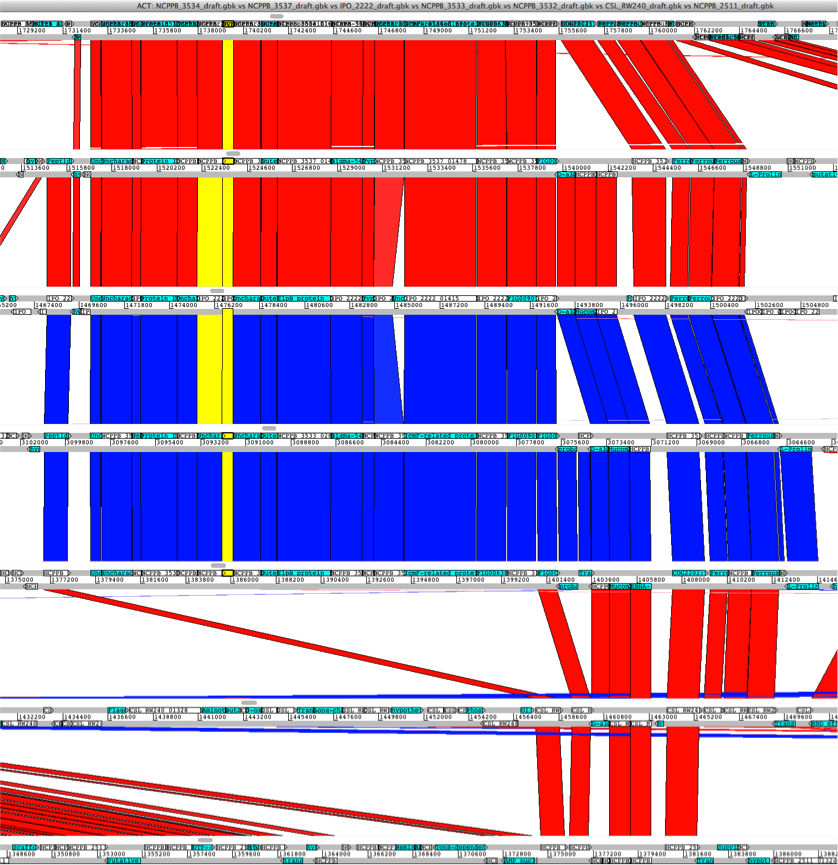
\includegraphics[width=1\textwidth]{images/t6ss}    
    \end{column}
  \end{columns}
\end{frame}